\section{Data Source and Characteristics}
\label{sec:targets}

This section fixes the data source, panel keys, and chronological constraints used throughout the project. Data pre-processing details (missing-value handling, normalisation, feature engineering) live in \cref{sec:eda}, which also contains the exploratory analysis.

\subsection{Source}

The dataset is the publicly released Kaggle competition \href{https://www.kaggle.com/competitions/ts-forecasting}{\emph{Hedge fund -- time-series forecasting}}, distributed as two parquet files (\texttt{train.parquet}, \texttt{test.parquet}) totalling approximately one gigabyte. The training partition spans $\mathtt{ts\_index}$ 1 to 3601, the held-out test partition continues from $\mathtt{ts\_index}$ 3602 to 4376. All identifiers, feature names, and underlying financial semantics are anonymised by the competition organiser.

\subsection{Panel keys and unit of analysis}

A row of the panel has primary keys
$(\mathtt{code},\mathtt{sub\_code},\mathtt{sub\_category},\mathtt{horizon},\mathtt{ts\_index})$.
We treat the 4-tuple
\[
s \;\equiv\; (\mathtt{code},\mathtt{sub\_code},\mathtt{sub\_category},\mathtt{horizon})
\]
as the natural \emph{series identifier}, and treat $\mathtt{ts\_index}$ as the time axis. There are 23 codes, 180 distinct sub-codes, 5 sub-categories, and 4 horizons in train, yielding 36{,}923 distinct series. Test uses a narrower sub-code support of 47 distinct values, which is a coverage shift rather than a schema mismatch (every test category level already exists in train).
\begin{figure}[h]
\centering
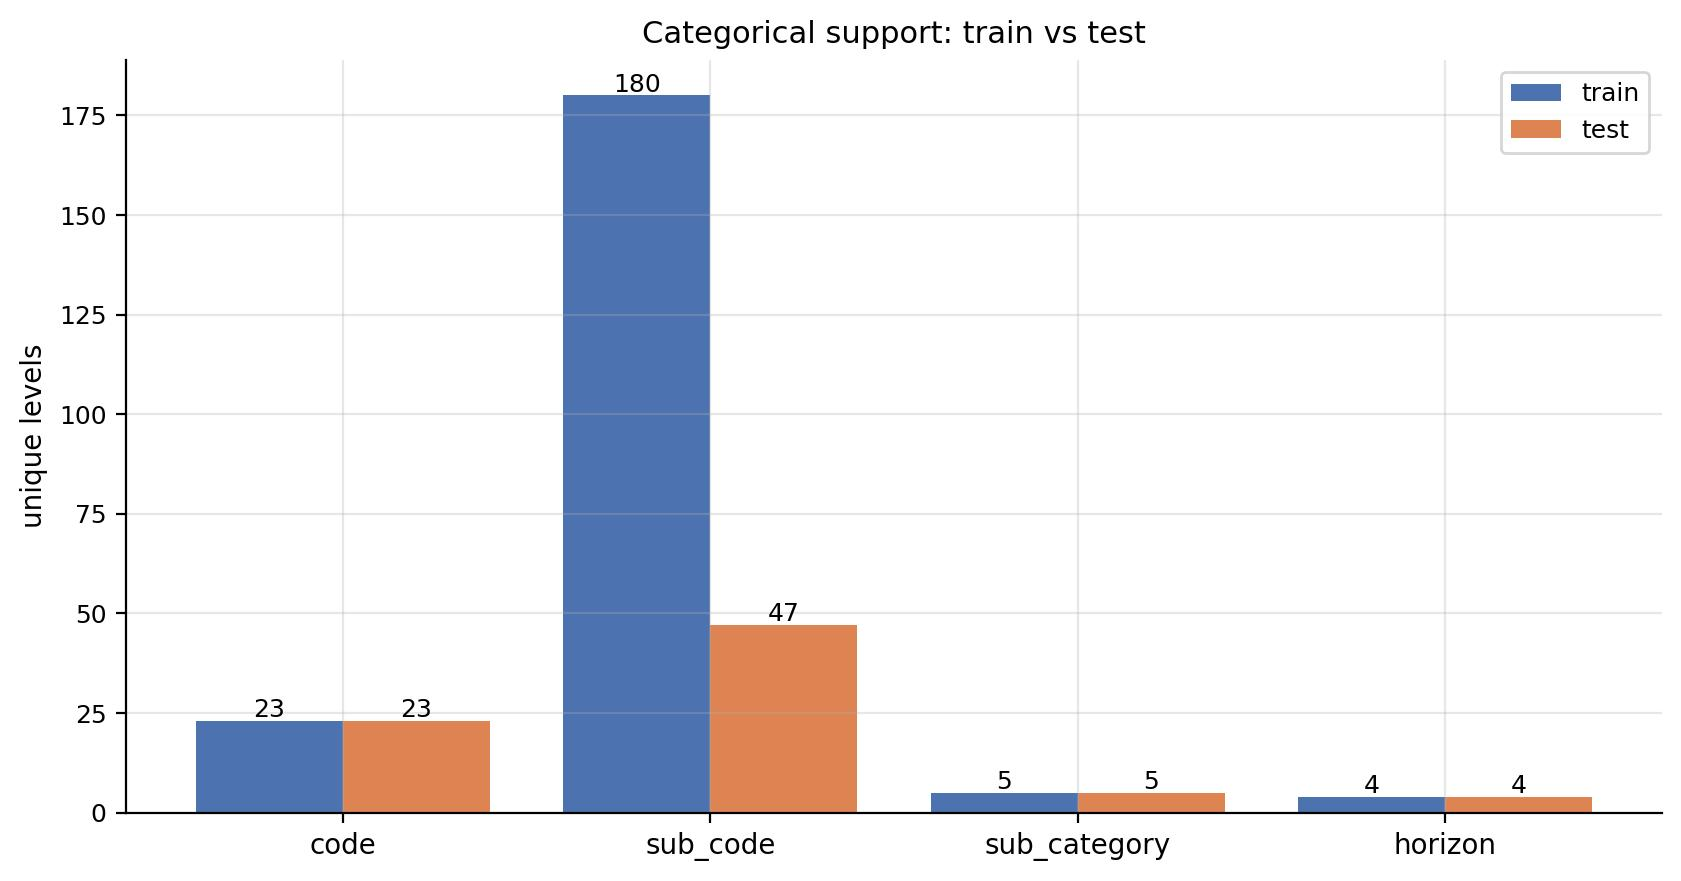
\includegraphics[width=0.85\linewidth]{figures/support_check.jpeg}
\caption{Comparison of categorical coverage between train and test sets, showing consistent schema but reduced sub\_code support in the test data.}
\label{fig:support_check}
\end{figure}

\subsection{The four horizons are coupled}

A naive reading of the schema would treat the four horizons of the same $(\mathtt{code},\mathtt{sub\_code},\mathtt{sub\_category})$ as four independent series, simply distinguished by an extra integer label. Two empirical facts in \cref{sec:eda} contradict this view:

\begin{enumerate}
  \item For approximately 1.21 million distinct $(\mathtt{code},\mathtt{sub\_code},\mathtt{sub\_category},\mathtt{ts\_index})$ tuples, all four horizons are simultaneously present (\cref{sec:multihorizon}).
  \item For the same triple, the target at horizon $k$ is closely approximated by the rolling sum of the $H=1$ target over the next $k$ steps:
  \[
    y^{H_k}_t \;\approx\; \sum_{i=0}^{k-1} y^{H_1}_{t+i}.
  \]
  We verify this on a stratified sample of 500 triples in \cref{sec:cumulation}, and find median Pearson correlations of 0.96, 0.94 and 0.91 at $k=3,10,25$ respectively.
\end{enumerate}

The practical consequence is that fitting four independent regressors per triple discards a strong constraint that the data construction itself imposes. We exploit this constraint in the H1-aggregation experiment scheduled for a later notebook.

\subsection{Chronological constraint}

The training partition runs over $\mathtt{ts\_index} \in [1, 3601]$ and the test partition over $[3602, 4376]$. Because test is a strict temporal suffix of train, any internal validation strategy must also be chronological, with all training points strictly preceding the validation points in time. Random or leave-one-series-out cross-validation would mix future information into earlier states and overstate generalisation.

We use a single canonical chronological partition throughout the project, fixed in the shared utilities at \texttt{cf.splits}:

\begin{itemize}
  \item \textbf{Train:} $\mathtt{ts\_index} \le 2880$.
  \item \textbf{Meta} (used only for fitting ensemble weights): $2880 < \mathtt{ts\_index} \le 3240$.
  \item \textbf{Holdout} (final scored window): $3240 < \mathtt{ts\_index} \le 3601$.
  \item \textbf{Test} ($\mathtt{ts\_index} \ge 3602$): unlabeled, used only for submission-style sanity checks.
\end{itemize}

The cutoff $\mathtt{ts\_index} = 2880$ matches the cutoff used in the midway report, preserving comparability with prior diagnostic figures. The meta/holdout boundary at 3240 places approximately one third of the post-cutoff window into the meta slice, leaving the remaining two thirds for final scoring.

\subsection{Eligibility for per-series studies}

Some classical model families (ARIMA, ARMA, MA, AR with order $\geq 2$) require a minimum training history. For per-series diagnostic studies we restrict attention to series that both cross the train/validation cutoff and have at least 120 training rows. There are 1{,}930 such \emph{eligible} series in the panel, roughly 5\% of the 36{,}923 total. Global pooled models and the H1-aggregation experiment use every row whose $\mathtt{ts\_index}$ falls inside the relevant split, so they are not constrained by per-series length.
